% fixture: tikz/loops-pdftex
% oracle: pdflatex
% tier: T3
% engine: document
% specials: compare
% covers: TikZ loops (topaths' loop, loop above, below, left and right: the target the start, looseness=8, min distance=5mm, every loop's -> and shorten >=1pt) on nodes and with labels, a loop on a small node (min distance), a loop whose target is another node (the start it is), edges with bend left between nodes, shorten < and shorten >
% issue: #352
\documentclass{article}
\usepackage{tikz}
\usetikzlibrary{arrows.meta,positioning}
\begin{document}
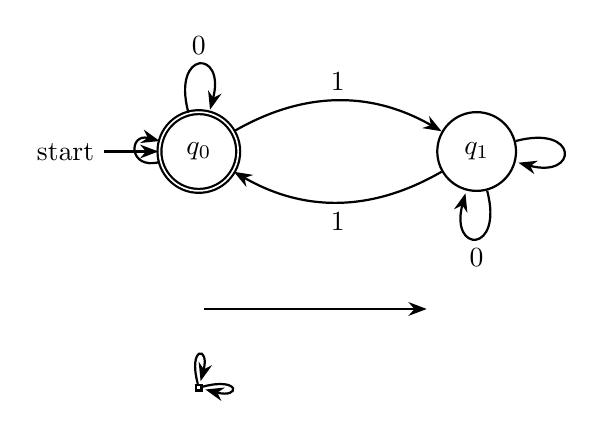
\begin{tikzpicture}[->, >=Stealth, node distance=2.5cm, thick,
                    state/.style={circle, draw, minimum size=1cm}]
  \node[state, double] (q0) {$q_0$};
  \node[state, right=of q0] (q1) {$q_1$};
  \draw (q0) edge[loop above] node {0} (q0)
        (q0) edge[bend left] node[above] {1} (q1)
        (q1) edge[bend left] node[below] {1} (q0)
        (q1) edge[loop below] node {0} (q1)
        (q1) edge[loop right] (q1)
        (q0) edge[loop left, looseness=4] (q0);
  \draw[<-] (q0) -- ++(-1.2,0) node[left] {start};
  \draw[shorten <=2pt, shorten >=3pt] (0,-2) -- (3,-2);
  \node[draw, inner sep=1pt] (p) at (0,-3) {};
  \draw (p) edge[loop above] (p) (p) edge[loop right] (q1);
\end{tikzpicture}
\end{document}
